\documentclass[tikz,border=10pt]{standalone}
\begin{document}
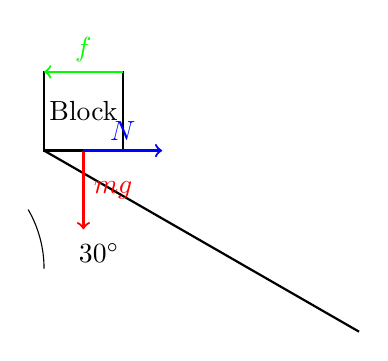
\begin{tikzpicture}

    % Defining the block
    \draw[thick] (0,0) rectangle (1,1);
    \node at (0.5,0.5) {Block};
    
    % Inclined plane
    \draw[thick] (0,0) -- (4,-2.3);
    
    % Showing angle
    \draw (0,-1.5) arc(0:30:1.5);
    \node at (0.7,-1.3) {$30^\circ$};
    
    % Forces acting on the block
    % Gravitational force    
    \draw[thick,->,red] (0.5,0) -- (0.5,-1) node[midway,right] {$mg$};
    
    % Normal force
    \draw[thick,->,blue] (0.5,0) -- (1.5,0) node[midway,above] {$N$};
    
    % Frictional force
    \draw[thick,->,green] (1,1) -- (0,1) node[midway,above] {$f$};

\end{tikzpicture}
\end{document}